\chapter{Преобразование алгебраических выражений}
\begin{definition}\term{Подобные слагаемые} (\emph{like terms}) — слагаемые с одинаковой буквенной частью, включая показатели степеней.\end{definition}
\begin{definition}\term{Разложение на множители} (\emph{factorization}) — представление выражения в виде произведения.\end{definition}
\begin{definition}\term{Тождество} (\emph{identity}) — равенство, верное при всех допустимых значениях переменных.\end{definition}
\begin{definition}\term{Область допустимых значений (ОДЗ)} (\emph{admissible values; domain of an expression}) — значения переменных, при которых исходное выражение имеет смысл.\end{definition}
\section*{Формулы сокращённого умножения}
\((a + b)^{2} = a^{2} + 2 ab + b^{2}\).\par
\((a - b)^{2} = a^{2} - 2 ab + b^{2}\).\par
\(a^{2} - b^{2} = (a - b) (a + b)\).\par
\section*{Правила преобразований}
Общий множитель: \(ab + ac = a (b + c)\). Подобные слагаемые складывают по коэффициентам: \(2 x + 3 x = 5 x\).\par
В дроби сокращают общие множители числителя и знаменателя, а не отдельные слагаемые.\par
После сокращения сохраняют запреты исходного выражения. Знаменатель не равен \(0\); под квадратным корнем стоит неотрицательное число.\par
Чтобы убрать корень из знаменателя вида \(\sqrt{a} - b\), можно умножить числитель и знаменатель на \(\sqrt{a} + b\), если преобразование допустимо.\par
{\small\textit{Пример: \(\frac{x^{2} - 1}{x - 1} = x + 1\), но только при \(x \ne  1\).}}\par

\Needspace{7\baselineskip}\section*{Задачи}
\begin{enumerate}[label={},leftmargin=3.2em,itemsep=10pt]
\Needspace{3\baselineskip}\item[\textbf{9.1.}] Раскрой скобки: \(3 (2 x - 5) - 2 (x + 1)\).
\Needspace{3\baselineskip}\item[\textbf{9.2.}] Приведи подобные: \(4 a - 3 b + 2 a + 5 b\).
\Needspace{3\baselineskip}\item[\textbf{9.3.}] Раскрой скобки: \((x + 3)^{2}\).
\Needspace{3\baselineskip}\item[\textbf{9.4.}] Раскрой скобки: \((2 x - 1) (2 x + 1)\).
\Needspace{3\baselineskip}\item[\textbf{9.5.}] Разложи на множители: \(6 x^{2} - 9 x\).
\Needspace{3\baselineskip}\item[\textbf{9.6.}] Разложи на множители: \(x^{2} - 16\).
\Needspace{3\baselineskip}\item[\textbf{9.7.}] Разложи на множители: \(x^{2} + 5 x + 6\).
\Needspace{3\baselineskip}\item[\textbf{9.8.}] Сократи \(\frac{x^{2} - 1}{x - 1}\). Укажи ограничения исходной дроби.
\Needspace{3\baselineskip}\item[\textbf{9.9.}] Упрости \(\frac{2}{x} + \frac{3}{2 x}\). Укажи ограничения.
\Needspace{3\baselineskip}\item[\textbf{9.10.}] Упрости \(\frac{a^{2} b}{ab^{2}}\). Укажи ограничения.
\Needspace{3\baselineskip}\item[\textbf{9.11.}] Упрости \(\frac{x^{2} - 4}{x^{2} + 4 x + 4}\). Укажи ограничения.
\Needspace{3\baselineskip}\item[\textbf{9.12.}] Упрости \(\frac{1}{\sqrt{5} - 2}\), избавившись от корня в знаменателе.
\Needspace{3\baselineskip}\item[\textbf{9.13.}] Из жизни. Билет стоит \(x\) рублей. Заказали \(3\) взрослых билета по полной цене и \(2\) детских по цене \(x - 100\) рублей. Составь и упрости выражение общей стоимости, если \(x > 100\).
\Needspace{3\baselineskip}\item[\textbf{9.14.}] Из жизни. У прямоугольной клумбы стороны \(x + 2\) и \(x + 5\) метров, где \(x > 0\). Вырази площадь многочленом.
\Needspace{3\baselineskip}\item[\textbf{9.15.}] Из жизни. Квадратную площадку со стороной \(x>0\) метров расширили на \(3\) м в каждом измерении. На сколько выросла её площадь?
\begin{center}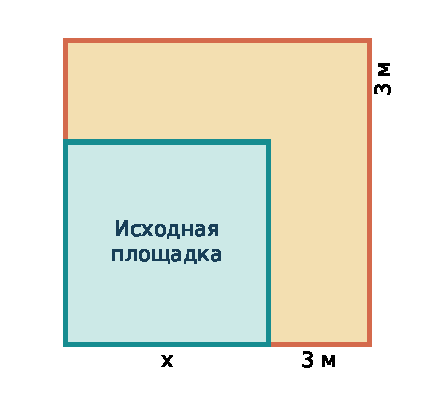
\includegraphics[width=.7\linewidth,height=45mm,keepaspectratio]{images/diagram-square.pdf}\end{center}
\Needspace{3\baselineskip}\item[\textbf{9.16.}\starmark] Упрости \(\frac{x^{2} - 9}{x^{2} - x - 6}\) и укажи ОДЗ исходного выражения.
\Needspace{3\baselineskip}\item[\textbf{9.17.}\starmark] Упрости: \((\frac{1}{x - 1} - \frac{1}{x + 1}) : (\frac{2}{x^{2} - 1})\).
\Needspace{3\baselineskip}\item[\textbf{9.18.}\starmark] Докажи тождество \((a + b)^{2} - (a - b)^{2} = 4 ab\) и проверь его при \(a = 103,\allowbreak b = 97\), не вычисляя квадраты больших чисел.
\Needspace{3\baselineskip}\item[\textbf{9.19.}] Докажите тождество \((a+b)^2+(a-b)^2=2a^2+2b^2\) для любых действительных \(a,b\).
\Needspace{3\baselineskip}\item[\textbf{9.20.}] Докажите, что при \(x\neq-1\) и \(x\neq1\) выполнено \(\frac1{x-1}-\frac1{x+1}=\frac2{x^2-1}\). Объясните, зачем нужны оба исключения.
\end{enumerate}
